\chapter{Proverb 26}

\begin{figure}
  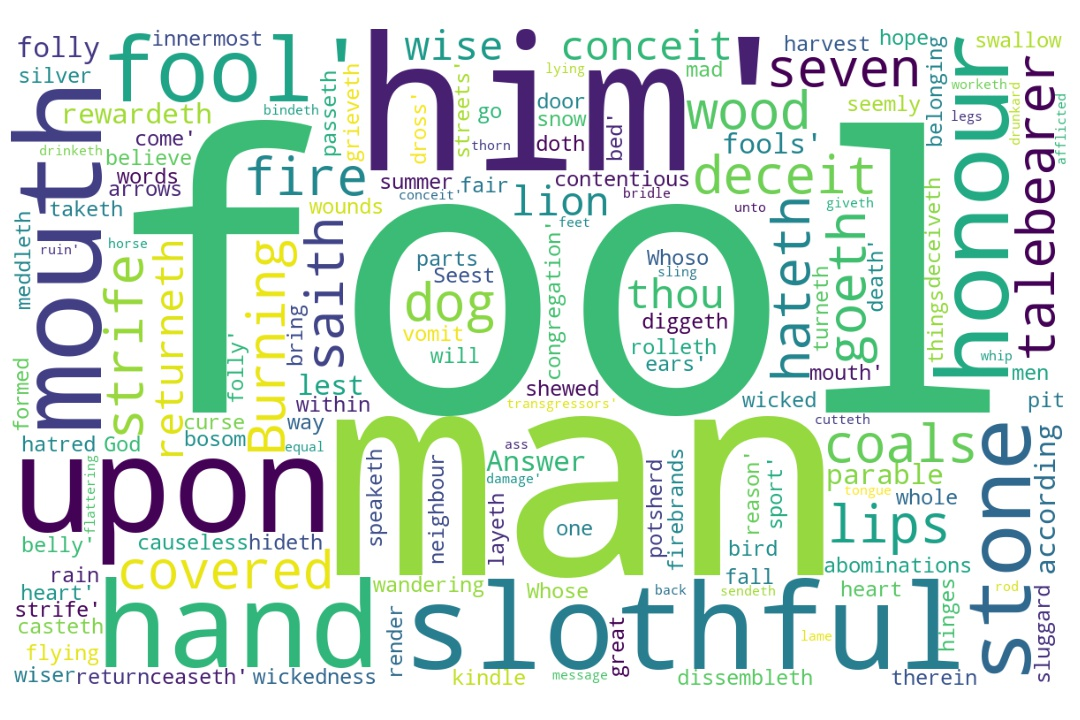
\includegraphics[width=\linewidth]{20OT-Proverbs/Proverb26-WordCloud.jpg}
  \caption{Proverb 26 Word Cloud}
  \label{fig:Proverb 26 word Cloud}
\end{figure}


\marginpar{\scriptsize \centering \fcolorbox{bone}{lime}{\textbf{CHARACTER OF A FOOL}}\\ (Proverb 26:1--28) \begin{compactenum}[I.][8]
    \item \textbf{Uncorrected} \index[scripture]{Proverbs!Pro 26:04}(Pro 26:4) -- one that stays uncorrected, and even worse is proud of that
    \item \textbf{Unreliable} \index[scripture]{Proverbs!Pro 26:06}(Pro 26:6)
    \item \textbf{Unteachable} \index[scripture]{Proverbs!Pro 26:07, 09}(Pro 26:7, 9)
    \item \textbf{Unworthy} \index[scripture]{Proverbs!Pro 26:08}(Pro 26:8) -- of course, we are ultimately all unworthy, but if nothing worthy of praise emerges in a life then perhaps ...
    \item \textbf{Unchangeable} \index[scripture]{Proverbs!Pro 26:11}(Pro 26:11)
    \item \textbf{Unmotivated} \index[scripture]{Proverbs!Pro 26:15}(Pro 26:15)
    \item \textbf{Uncaring} \index[scripture]{Proverbs!Pro 26:28}(Pro 26:28)
\end{compactenum}}

\marginpar{\scriptsize \centering \fcolorbox{bone}{yellow}{\textbf{THE CASTLES OF CONCEIT}}\\ (Proverb 26:1--28)\\The rich, powerful, highly educated: \\
Introduction: see \href{https://www.skywardcoaching.com/single-post/2016/07/13/the-seven-habits-of-highly-uncoachable-people}{The Seven Habits of Highly Un/Coachable People}. Plenty of scriptural examples, such as, Pharaoh, Saul, Nabal, and anyone who rejects the gospel ...
\begin{compactenum}[I.][8]
    \item Think themselves \textbf{Invulnerable and Indestructible} %\index[scripture]{Proverbs!Pro 26:04}(Pro 26:4) -- one that stays uncorrected, and even worse is proud of that
    \item Think themselves \textbf{Impressive}
    \item Think themselves \textbf{Indispensible}
    \item Acts \textbf{Independent} (from God and truth)
    \item Are \textbf{Incorrigible}
    \item Are \textbf{Impetuous} (uncoachable and uncorrectible)
    \item Instead are \textbf{Insecure \& Insubstantial}
\end{compactenum}}

\footnote{\textcolor[cmyk]{0.99998,1,0,0}{\hyperlink{TOC}{Return to end of Table of Contents.}}}\footnote{\href{https://www.audioverse.org/english/audiobibles/books/ENGKJV/O/Prov/1}{\textcolor[cmyk]{0.99998,1,0,0}{Proverbs Audio}}}\textcolor[cmyk]{0.99998,1,0,0}{As snow \fcolorbox{bone}{bone}{in} summer, and as rain \fcolorbox{bone}{bone}{in} harvest, so honour is not seemly for a fool.}
[2] \textcolor[cmyk]{0.99998,1,0,0}{As the bird by wandering, as the swallow by flying, so the curse causeless shall not come.}
[3] \textcolor[cmyk]{0.99998,1,0,0}{A whip for the horse, a bridle for the ass, and a rod for the fool's back.}
[4] \textcolor[cmyk]{0.99998,1,0,0}{Answer not a fool according to his \fcolorbox{bone}{lime}{folly}, lest thou also be like unto him.}
[5] \textcolor[cmyk]{0.99998,1,0,0}{Answer a fool according to his folly, lest he be wise \fcolorbox{bone}{bone}{in} his own conceit.}
[6] \textcolor[cmyk]{0.99998,1,0,0}{He that sendeth a message \fcolorbox{bone}{lime}{by the hand of a fool} cutteth off the feet, \emph{and} drinketh damage.}
[7] \textcolor[cmyk]{0.99998,1,0,0}{The legs of the lame are not equal: so \emph{is} a parable \fcolorbox{bone}{lime}{in the mouth} \fcolorbox{bone}{lime}{of fools}.}
[8] \textcolor[cmyk]{0.99998,1,0,0}{As he that bindeth a stone \fcolorbox{bone}{bone}{in} a sling, so \emph{is} he that giveth \fcolorbox{bone}{lime}{honour to a fool}.}
[9] \textcolor[cmyk]{0.99998,1,0,0}{\emph{As} a thorn goeth up into the hand of a drunkard, so \emph{is} a parable \fcolorbox{bone}{bone}{in} the mouth of fools.}
[10] \textcolor[cmyk]{0.99998,1,0,0}{The great \emph{God} that formed all \emph{things} both rewardeth the fool, and rewardeth \fcolorbox{bone}{MYGOLD}{transgressors}.}
[11] \textcolor[cmyk]{0.99998,1,0,0}{As a dog returneth to his vomit, \emph{so} a fool \fcolorbox{bone}{lime}{returneth} to his folly.}
[12] \textcolor[cmyk]{0.99998,1,0,0}{Seest thou a man wise \fcolorbox{bone}{bone}{in} his own conceit? \emph{there} \emph{is} more hope of a fool than of him.}
[13] \textcolor[cmyk]{0.99998,1,0,0}{The slothful \emph{man} saith, \emph{There} \emph{is} a lion \fcolorbox{bone}{bone}{in} the way; a lion \emph{is} \fcolorbox{bone}{bone}{in} the streets.}
[14] \textcolor[cmyk]{0.99998,1,0,0}{\emph{As} the door turneth upon his hinges, so \emph{doth} the slothful upon his bed.}
[15] \textcolor[cmyk]{0.99998,1,0,0}{The slothful hideth his hand \fcolorbox{bone}{bone}{in} \emph{his} bosom; it \fcolorbox{bone}{lime}{grieveth him} to bring it again to his mouth.}
[16] \textcolor[cmyk]{0.99998,1,0,0}{The sluggard \emph{is} wiser \fcolorbox{bone}{bone}{in} his own conceit than seven men that can render a reason.}
[17] \textcolor[cmyk]{0.99998,1,0,0}{He that passeth by, \emph{and} meddleth with strife \emph{belonging} not to him, \emph{is} \emph{like} one that taketh a dog by the ears.}
[18] \textcolor[cmyk]{0.99998,1,0,0}{As a mad \emph{man} who casteth firebrands, arrows, and death,}
[19] \textcolor[cmyk]{0.99998,1,0,0}{So \emph{is} the man \emph{that} deceiveth his neighbour, and saith, Am not I \fcolorbox{bone}{bone}{in} sport?}
[20] \textcolor[cmyk]{0.99998,1,0,0}{Where no wood is, \emph{there} the fire goeth out: so where \emph{there} \emph{is} no talebearer, the strife ceaseth.}
[21] \textcolor[cmyk]{0.99998,1,0,0}{\emph{As} coals \emph{are} to burning coals, and wood to fire; so \emph{is} a contentious man to kindle strife.}
[22] \textcolor[cmyk]{0.99998,1,0,0}{The words of a talebearer \emph{are} as wounds, and they go down into the innermost parts of the belly.}
[23] \textcolor[cmyk]{0.99998,1,0,0}{Burning lips and a wicked heart \emph{are} \emph{like} a potsherd covered with silver dross.}
[24] \textcolor[cmyk]{0.99998,1,0,0}{He that hateth dissembleth with his lips, and layeth up deceit within him;}
[25] \textcolor[cmyk]{0.99998,1,0,0}{When he speaketh fair, believe him not: for \emph{there} \emph{are} seven abominations \fcolorbox{bone}{bone}{in} his heart.}\footnote{These seven abominations are listen in Proverbs 6:16-19:
\begin{compactenum}
\item A Proud Look
\item A Lying Tongue
\item Hands that Shed Innocent Blood
\item A Heart that Deviseth Wicked Imaginations
\item Feet that a swift to run to mischief
\item A False Witness
\item He that sow discord among brethren
\end{compactenum}
\textbf{Proverbs 6:16-19} - These six things doth the LORD hate: yea, seven are an abomination unto him: [17] A proud look, a lying tongue, and hands that shed innocent blood, [18] An heart that deviseth wicked imaginations, feet that be swift \fcolorbox{bone}{bone}{in} running to mischief, [19] A false witness that speaketh lies, and he that soweth discord among brethren.}
[26] \textcolor[cmyk]{0.99998,1,0,0}{\emph{Whose} hatred is covered by deceit, his wickedness shall be shewed before the \emph{whole} congregation.}
[27] \textcolor[cmyk]{0.99998,1,0,0}{Whoso diggeth a pit shall fall therein: and he that rolleth a stone, it will return upon him.}\footnote{\textbf{Proverb 1:31} -  Therefore shall they eat of the fruit of their own way, and be filled with their own devices.}\footnote{\textbf{Jeremiah 18:12} - And they said, There is no hope: but we will walk after our own devices, and we will every one do the imagination of his evil heart.}
[28] \textcolor[cmyk]{0.99998,1,0,0}{A \fcolorbox{bone}{lime}{lying tongue} hateth \emph{those} \emph{that} \emph{are} afflicted by it; and a flattering mouth worketh ruin.}


